\documentclass [11pt,twoside]{article}
\usepackage[utf8]{inputenc}
\usepackage[T1]{fontenc}

%Page margins, header and footer positions
\usepackage{geometry}
 \geometry{
 a4paper,
 total={210mm,297mm},
 left=25mm,
 right=25mm,
 top=30mm,
 bottom=25mm,
 headsep=7mm}

\interfootnotelinepenalty=10000

%To display filling dots in the TOC for all entries
\usepackage[titles]{tocloft}
\renewcommand{\cftsecleader}{\cftdotfill{\cftdotsep}}

%Define new header and footer style
\usepackage{fancyhdr}

\pagestyle{fancy}
\fancyhf{}
\lhead{\color{Gray}{\small{Travlendar+ project by Daverio Fiorillo}}}
\lfoot{\textcolor{Gray}{\small{Copyright © 2017, Daverio Fiorillo – All rights reserved}}}
\rfoot{\textcolor{Gray}{\thepage}}
\renewcommand{\headrulewidth}{0pt}

%PACKAGES
\usepackage{wasysym}
\usepackage{pifont}
\usepackage{float}

\newcommand{\supported}{\ding{52}\xspace}
\newcommand{\unsupported}{\ding{55}\xspace}
\newcommand{\partsupported}{\textcolor{black!40}{\ding{52}}\xspace}
\newcommand{\lowsupported}{\textcolor{black!20}{\ding{52}}\xspace}
\newcommand{\unknowsupported}{\textbf{?}\xspace}

%Font: Times
\usepackage{times}
%Change monospaced font
\renewcommand{\ttdefault}{lmtt}

%tables
\usepackage{tabu}
\usepackage{tabularx}
\usepackage{ltablex}
\usepackage{longtable}
\usepackage{float} % To allow the use of H modifier in long tables

%landscape mode
\usepackage{pdflscape}
\usepackage{rotating}
\usepackage{caption}

%make landscape mode be sensitive to even and odd pages
%start
\def\myrotate{\ifodd\c@page\else-\fi 90}
\makeatletter
\global\let\orig@begin@landscape=\landscape%
\global\let\orig@end@landscape=\endlandscape%
\gdef\@true{1}
\gdef\@false{0}
\gdef\landscape{%
    \global\let\within@landscape=\@true%
    \orig@begin@landscape%
}%
\gdef\endlandscape{%
    \orig@end@landscape%
    \global\let\within@landscape=\@false%
}%
\@ifpackageloaded{pdflscape}{%
    \gdef\pdf@landscape@rotate{\PLS@Rotate}%
}{
    \gdef\pdf@landscape@rotate#1{}%
}
\let\latex@outputpage\@outputpage
\def\@outputpage{
    \ifx\within@landscape\@true%
        \if@twoside%
            \ifodd\c@page%
                \gdef\LS@rot{\setbox\@outputbox\vbox{%
                    \pdf@landscape@rotate{-90}%
                    \hbox{\rotatebox{90}{\hbox{\rotatebox{180}{\box\@outputbox}}}}}%
                }%
            \else%
                \gdef\LS@rot{\setbox\@outputbox\vbox{%
                    \pdf@landscape@rotate{+90}%
                    \hbox{\rotatebox{90}{\hbox{\rotatebox{0}{\box\@outputbox}}}}}%
                }%
            \fi%
        \else%
            \gdef\LS@rot{\setbox\@outputbox\vbox{%
                \pdf@landscape@rotate{+90}%
                \hbox{\rotatebox{90}{\hbox{\rotatebox{0}{\box\@outputbox}}}}}%
            }%
        \fi%
    \fi%
    \latex@outputpage%
}
\makeatother
%end

%graphics
\usepackage{graphicx}
\usepackage[dvipsnames, table]{xcolor}
%If you upload images from PC, you need to insert code for the path here (different for Windows and Unix OS)

%References
%\usepackage{xpatch}
%\usepackage[backend=biber, style=numeric, citestyle=numeric, sorting=none]{biblatex}
%\addbibresource{main.bib}

%Other
\usepackage{ifthen}
\usepackage{xspace}
\usepackage{enumitem}
\usepackage{amssymb}
\usepackage[pdftex, colorlinks]{hyperref}
\newcommand{\comment}[1]{{\color{Red}$\blacktriangleright$ Comment: #1 $\blacktriangleleft$}}


% Some utilities\ldots
\usepackage{soul}
\usepackage{tikz}

\usetikzlibrary{calc}
\usetikzlibrary{decorations.pathmorphing}


\makeatletter

\newcommand{\defhighlighter}[3][]{%
  \tikzset{every highlighter/.style={color=#2, fill opacity=#3, #1}}%
}

\defhighlighter{yellow}{.5}

\newcommand{\highlight@DoHighlight}{
  \fill [ decoration = {random steps, amplitude=1pt, segment length=15pt}
        , outer sep = -15pt, inner sep = 0pt, decorate
       , every highlighter, this highlighter ]
        ($(begin highlight)+(0,8pt)$) rectangle ($(end highlight)+(0,-3pt)$) ;
}

\newcommand{\highlight@BeginHighlight}{
  \coordinate (begin highlight) at (0,0) ;
}

\newcommand{\highlight@EndHighlight}{
  \coordinate (end highlight) at (0,0) ;
}

\newdimen\highlight@previous
\newdimen\highlight@current

\DeclareRobustCommand*\highlight[1][]{%
  \tikzset{this highlighter/.style={#1}}%
  \SOUL@setup
  %
  \def\SOUL@preamble{%
    \begin{tikzpicture}[overlay, remember picture]
      \highlight@BeginHighlight
      \highlight@EndHighlight
    \end{tikzpicture}%
  }%
  %
  \def\SOUL@postamble{%
    \begin{tikzpicture}[overlay, remember picture]
      \highlight@EndHighlight
      \highlight@DoHighlight
    \end{tikzpicture}%
  }%
  %
  \def\SOUL@everyhyphen{%
    \discretionary{%
      \SOUL@setkern\SOUL@hyphkern
      \SOUL@sethyphenchar
      \tikz[overlay, remember picture] \highlight@EndHighlight ;%
    }{%
    }{%
      \SOUL@setkern\SOUL@charkern
    }%
  }%
  %
  \def\SOUL@everyexhyphen##1{%
    \SOUL@setkern\SOUL@hyphkern
    \hbox{##1}%
    \discretionary{%
      \tikz[overlay, remember picture] \highlight@EndHighlight ;%
    }{%
    }{%
      \SOUL@setkern\SOUL@charkern
    }%
  }%
  %
  \def\SOUL@everysyllable{%
    \begin{tikzpicture}[overlay, remember picture]
      \path let \p0 = (begin highlight), \p1 = (0,0) in \pgfextra
        \global\highlight@previous=\y0
        \global\highlight@current =\y1
      \endpgfextra (0,0) ;
      \ifdim\highlight@current < \highlight@previous
        \highlight@DoHighlight
        \highlight@BeginHighlight
      \fi
    \end{tikzpicture}%
    \the\SOUL@syllable
    \tikz[overlay, remember picture] \highlight@EndHighlight ;%
  }%
  \SOUL@
}

\makeatother

% Common abbrev. are set as commands to ensure proper spacing after the dot
\RequirePackage{xspace}
\newcommand{\ie}{i.e.\@\xspace}
\newcommand{\aka}{a.k.a.\@\xspace}
\newcommand{\Ie}{I.e.\@\xspace}
\newcommand{\cf}{cf.\@\xspace}
\newcommand{\Cf}{Cf.\@\xspace}
\newcommand{\eg}{e.g.\@\xspace}
\newcommand{\Eg}{E.g.\@\xspace}
\newcommand{\etal}{et al.\@\xspace}
\newcommand{\etc}{etc.\@\xspace}
\newcommand{\wrt}{w.r.t.\@\xspace}
\newcommand{\Wrt}{W.r.t.\@\xspace}



\date{}


\begin{document}

%TITLE PAGE

\begin{titlepage}


%LOGO

{\begin{table}[t!]
\centering
\begin{tabu} to \textwidth { X[1.3,r,p] X[1.7,l,p] }
\textcolor{Blue}
{\textbf{\small{Travlendar+ project Daverio Fiorillo}}} & 
\includegraphics[scale=0.5]{Images/PolimiLogo}
\end{tabu}
\end{table}}~\\ [7cm]

%TITLE 

\begin{flushleft}

%Replace the text string with your title
{\textcolor{Blue}{\textbf{\Huge{Requirement Analysis and Specification
        Document}}}} \\ [1cm]

\end{flushleft}

\end{titlepage}

%Define deliverable specific info
%Replace cell contents where needed
\begin{table}[h!]
\begin{tabu} to \textwidth { X[0.3,r,p] X[0.7,l,p] }
\hline

\textbf{Deliverable:} & RASD\\
\textbf{Title:} & Requirement Analysis and Verification Document \\
\textbf{Authors:} & Daverio Fiorillo \\
\textbf{Version:} & 1.0 \\ 
\textbf{Date:} & 29-October-2017 \\
\textbf{Download page:} & https://github.com/FiorixF1/DaverioFiorillo.git \\
\textbf{Copyright:} & Copyright © 2017, Daverio Fiorillo – All rights reserved \\
\hline
\end{tabu}
\end{table}




\setcounter{page}{2}

%------------------------------------------------------------------------------------------------------------------------------------------------
\newpage
\begin{verse}
	Many endeavors require scheduling meetings at various locations all across a city or a region (e.g., around Lombardy), whether for work or personal reasons (e.g., meeting the CEO of a partner company, going to the gym, taking children to practice, etc.). The goal of this project is to create a calendar-based application that: (i) automatically computes and accounts for travel time between appointments to make sure that the user is not late for appointments; and (ii) supports the user in his/her travels, for example by identifying the best mobility option (e.g., use the train from A to B and then the metro to C), buying public transportation tickets, or by locating the nearest bike of a bike sharing system. Users can create meetings, and when meetings are created at locations that are unreachable in the allotted time, a warning is created. As mentioned, the application should also suggest travel means depending on the appointment (e.g., perhaps you bike to the office in the morning, but the bus is a better choice between a pair of afternoon meetings, and a car – either personal, or of a car-sharing system – is best to take children to practice) and the day (e.g., the app should suggest that you leave your home via car in the morning because meetings during a strike day will not be doable via public transportation; it could also take into account the weather forecast, and avoid biking during rainy days). Travlendar+ should allow users to define various kinds of user preferences. It should support a multitude of travel means, including walking, biking (own or shared), public transportation (including taxis), driving (own or shared), etc. A particular user may globally activate or deactivate each travel means (e.g., a user who cannot drive would deactivate driving). A user should also be able to provide reasonable constraints on different travel means (e.g., walking distances should be less than a given distance, or public transportation should not be used after a given time of day). Users should also be able, if they wish to, to select combinations of transportation means that minimize carbon footprint. Additional features could also be envisioned, for instance allowing a user to specify a flexible "lunch". For instance, a user could be able to specify that lunch must be possible every day between 11:30- 2:30, and it must be at least half an hour long, but the specific timing is flexible. The app would then be sure to reserve at least 30 minutes for lunch each day. Similarly, other types of breaks might be scheduled in a customizable way
\end{verse}
%------------------------------------------------------------------------------------------------------------------------------------------------
\newpage
\addcontentsline{toc}{section}{Table of Contents}
\tableofcontents
\newpage
\addcontentsline{toc}{section}{List of Figures}
\listoffigures
\addcontentsline{toc}{section}{List of Tables}
\listoftables

%------------------------------------------------------------------------------------------------------------------------------------------------
\clearpage
{\color{Blue}{\section{Introduction}}}
\label{sect:introduction}
\subsection{Purpose}
The following document is the Requirement Analysis and Specification Document (RASD) for the formalization and description of all the needed features, constraints and recommendations that will constitute the proposed system.

The paper will focus on the elicitation and analysis of all functional and nonfunctional requirements, also verified by automated logic verification software (Alloy Analyzer [MIT]) and supported by UML schemes and scenarios.
The provided document will also include a concise analysis of the environment and it tries to clarify all the interaction among system parts and external world.

The target audiences of this document are all the stakeholders involved in the development of the system and it can be used as contractual base for the project.


\subsection{Scope}

\subsubsection{System description}

The system that would be developed is a calendar-based application that provides support for planning of appointments, automating the travel arrangement process according to the user preferences.
The system will be able to plan travel routes choosing transport options among public and private means, including trains, trams, taxis, bicycles, bike and car sharing, owned automobile and others. Therefore, the system will provide a set of possible route options, trying to minimize travel times, route length, carbon footprint or number of changes.

Also, it will have to recollect travel informations on public transportations and travelling conditions from different external sources.
Beside, the application will give the possibility to users to register themselves, allowing them to access a series of extra features, including the possibility of setting personal preferences and backup personal agenda and routes.

User preferences include the possibility to set travel pauses, flexible launch (30 minute of travel pause between 11.30-14.30), enabling and disabling certains types of transportation means in a specific period of the day or anytime and in addition it will give the possibility to user to create profiles of preferences and link them to single appointments)
Finally, system should be capable to interacting with any type of external public transportation service, although it will focus on make available them in the city of Milan.

\subsubsection{World Phenomena}

Many public transport service companies offers the possibility to obtains informations on timetables, routes, stations and status of services in aggregate way providing public Application Public Interfaces (APIs). Thus it is guaranteed the theoretical possibility to make queries in any moment and get the latest valid informations on transports.

Others doesn’t offer the same possibilities; for instance Trenitalia hasn’t yet a public API, but there are different opensource projects that allow to fill the gap.

Moreover, a lot of web mapping services makes available public APIs too. In this case it is possible to get GPS location from an address or vice-versa, or update a portion of map and even process a route given a starting point and a destination.
All the required supported companies provide aforementioned services.

\subsubsection{Goals}
%what you write here is a comment that is not shown in the final text
\begin{itemize}
	\item[G1] Allow the user to add an appointment
	\subitem[G1.1] The user can add the date of the appointment through a calendar
	\subitem[G1.2] The user can select the location through a map
	\subitem[G1.3] The appointment must be processed by the system
	\item[G2] - Provide a route to the user for reaching the appointments
	\subitem[G2.1] The user must reach on time his/her appointments
	\subitem[G2.2] The user can choose the starting location and time of the route
	\subitem[G2.3] Generate routes according to the preferences of the user
	\subitem[G2.4] The application provides a route for each objective, minimizing each of these attributes: length, duration, number of changes, carbon footprint
	\subitem[G2.5] Always provide a route
	\subitem[G2.6] During strike days, public transportation must not be available
	\subitem[G2.7] Report unfavorable weather conditions
	\subitem[G2.8] Update unfavorable weather conditions
	\subitem[G2.9] The user can save one route among the shown ones
	\item[G3] Allow the user to sign up into the application
	\subitem[G3.1] The registration must allow the univocal recognition of the user
	\item[G4] Allow the user to log in
	\subitem[G4.1] The system allow the login through e-mail and password
	\subitem[G4.2] The application allow the login through telephone number
	\item[G5] Allow the user to add his own preferences
	\subitem[G5.1] The user must be logged
	\subitem[G5.2] The preferences are synchronized between the application and the database
	\subitem[G5.3] The user can chose the available transport means
	\subitem[G5.4] The user can add a priority to the means of transport
	\subitem[G5.5] The user can add the maximum length of routes on foot or by bicycle
	\subitem[G5.6] For each vehicle the user can choose a time slot of validity
	\subitem[G5.7] The user can set Flexible Lunch
	\subitem[G5.8] The user can add breaks for fixed moments of the day
	\subitem[G5.9] The user can add a private car or bicycle
	\subitem[G5.10] The user can organize his preferences in “Preferences Profiles"
	\item[G6] Allow the user to manage his account
	\subitem[G6.1] The user must be able to remove appointments and routes
	\subitem[G6.2] The user must be able to modify appointments and routes
	\subitem[G6.3] The user must be able to delete his account
	\item[G7] Allow the user to report events and disservices 
	\subitem[G7.1] The user can report strikes using the application
	\subitem[G7.2] The user can report faults, malfunctions and suggestions
\end{itemize}

\subsection{Definitions, Acronyms, Abbreviations}

\subsubsection{Definitions}
\begin{itemize}
	\item API(s) : Application Program Interface(s)
	\item RASD : Requirement Analysis Specification Document
	\item Appointment: location the user has to reach at a fixed date and time
	\item Route: journey between two appointments, it is composed by a series of paths
	\item Path: part of a route traversed with a specific mean of transport
\end{itemize}


\subsubsection{Acronyms}
\begin{itemize}
	\item UI: User Interface
\end{itemize}

\subsubsection{Abbreviations}
\begin{itemize}
	\item MA (Mobile Application): part of the system
	\item PT: Public Transportation
\end{itemize}

\subsection{Revision history}




\subsection{References}


\begin{itemize}
	\item Specification Document assigned: \texttt{“Mandatory\_Project\_Assignments.pdf”}
	\item Software Requirements Specification Guidelines : IEEE 830-1998
	\item Alloy Website: \url{http://alloy.mit.edu/alloy/}
\end{itemize}

\subsection{Document Structure}

The document is composed of six different parts.

\begin{enumerate}
	
	\item The introduction has the objective to support the reader into the reading of the document providing a brief description of the problem and the actual technological landscape description. It also include a list of definition, abbreviations and acronyms commonly employed through the rest of the document.
	\item The second part offers an overall description of the system, then focused on the boundaries that divide the system from world, especially inspecting all interactions on shared phenomena. In addition, it is provided a short description of users. FInally, it is listed and described a set of core functionalities that will be supported and assumptions.
	\item The third part provides a more complex and detailed description of functionalities, also in terms of requirement. This part is addressed specifically to development team
	\item This section provides an Alloy model for verification of goals through a formal analysis of requirements and domain assumption. This is beneficial in assuring the consistency of the model. It also provide a representation of the world and system.
	\item The fifth part provides the effort spent in term of time involved into the project by the authors.
	In the last part, there are references to external sources.
	
\end{enumerate}



%------------------------------------------------------------------------------------------------------------------------------------------------
\clearpage
{\color{Blue}{\section{Overall Description}}}
\label{sect:overview}

\begin{sidewaysfigure}
\centering
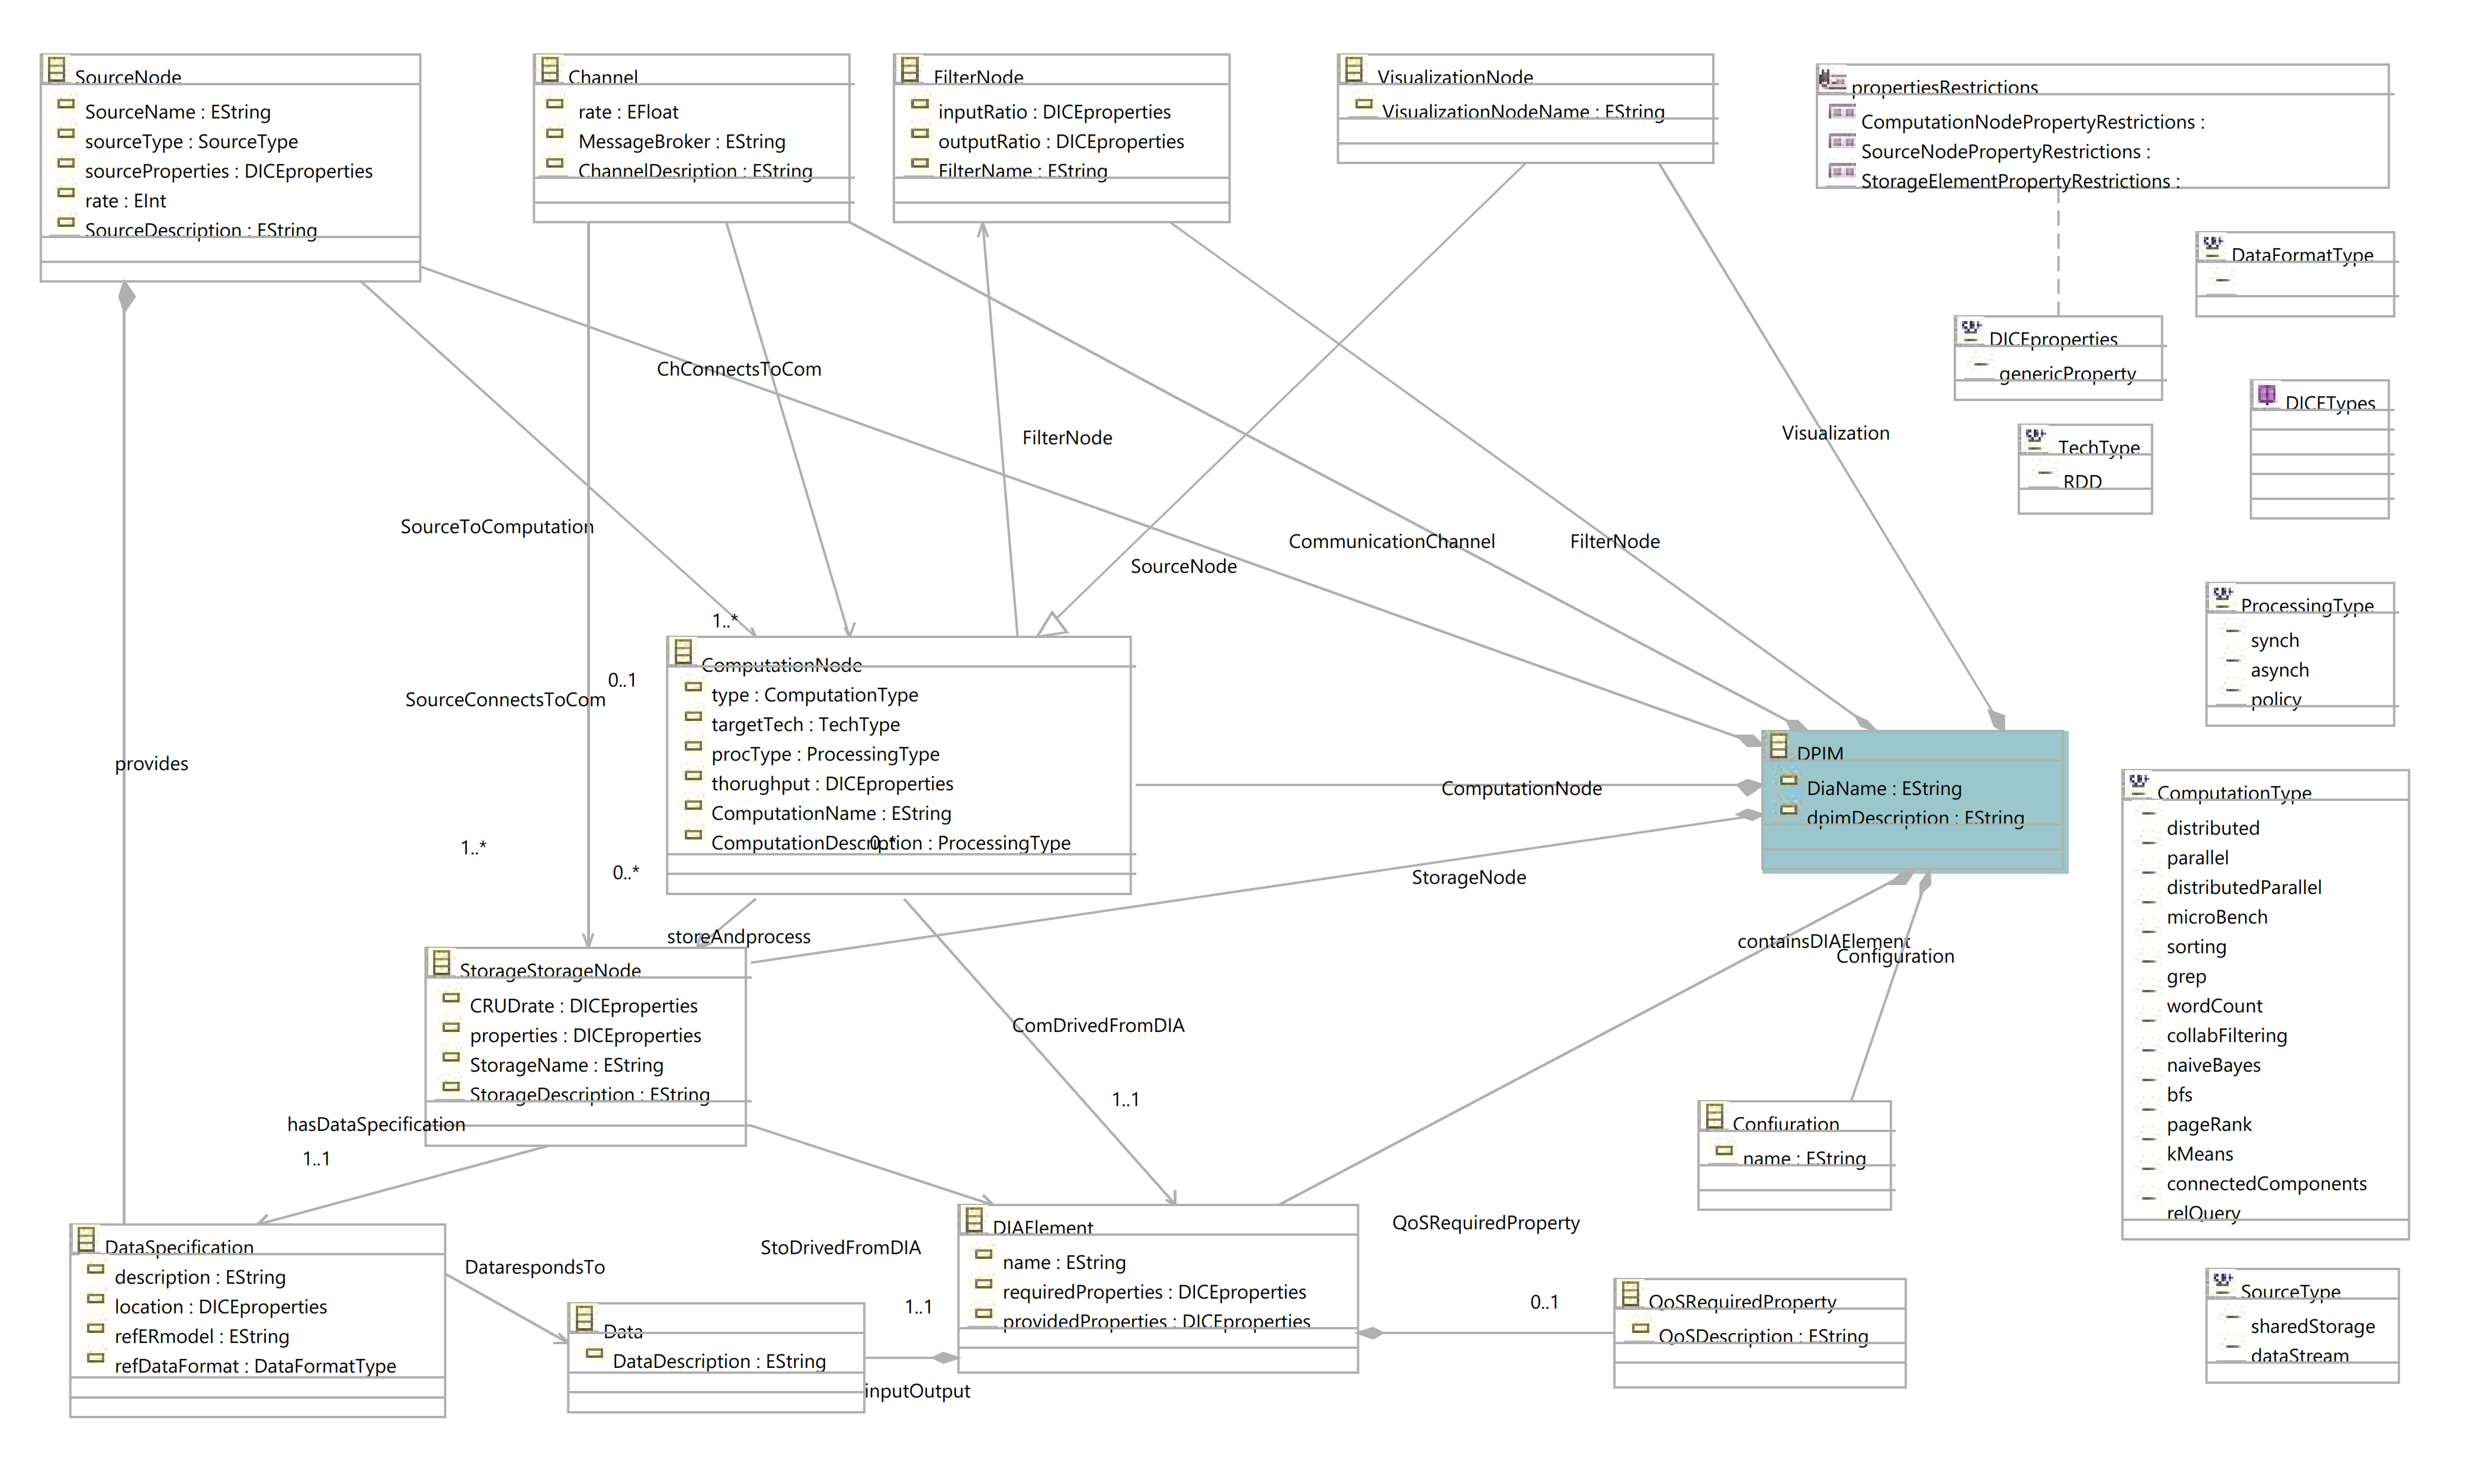
\includegraphics[width=\textwidth]{Images/11.png}
\caption{\label{fig:metamodel}DICE DPIM metamodel.}
\end{sidewaysfigure}

\begin{figure}
\centering
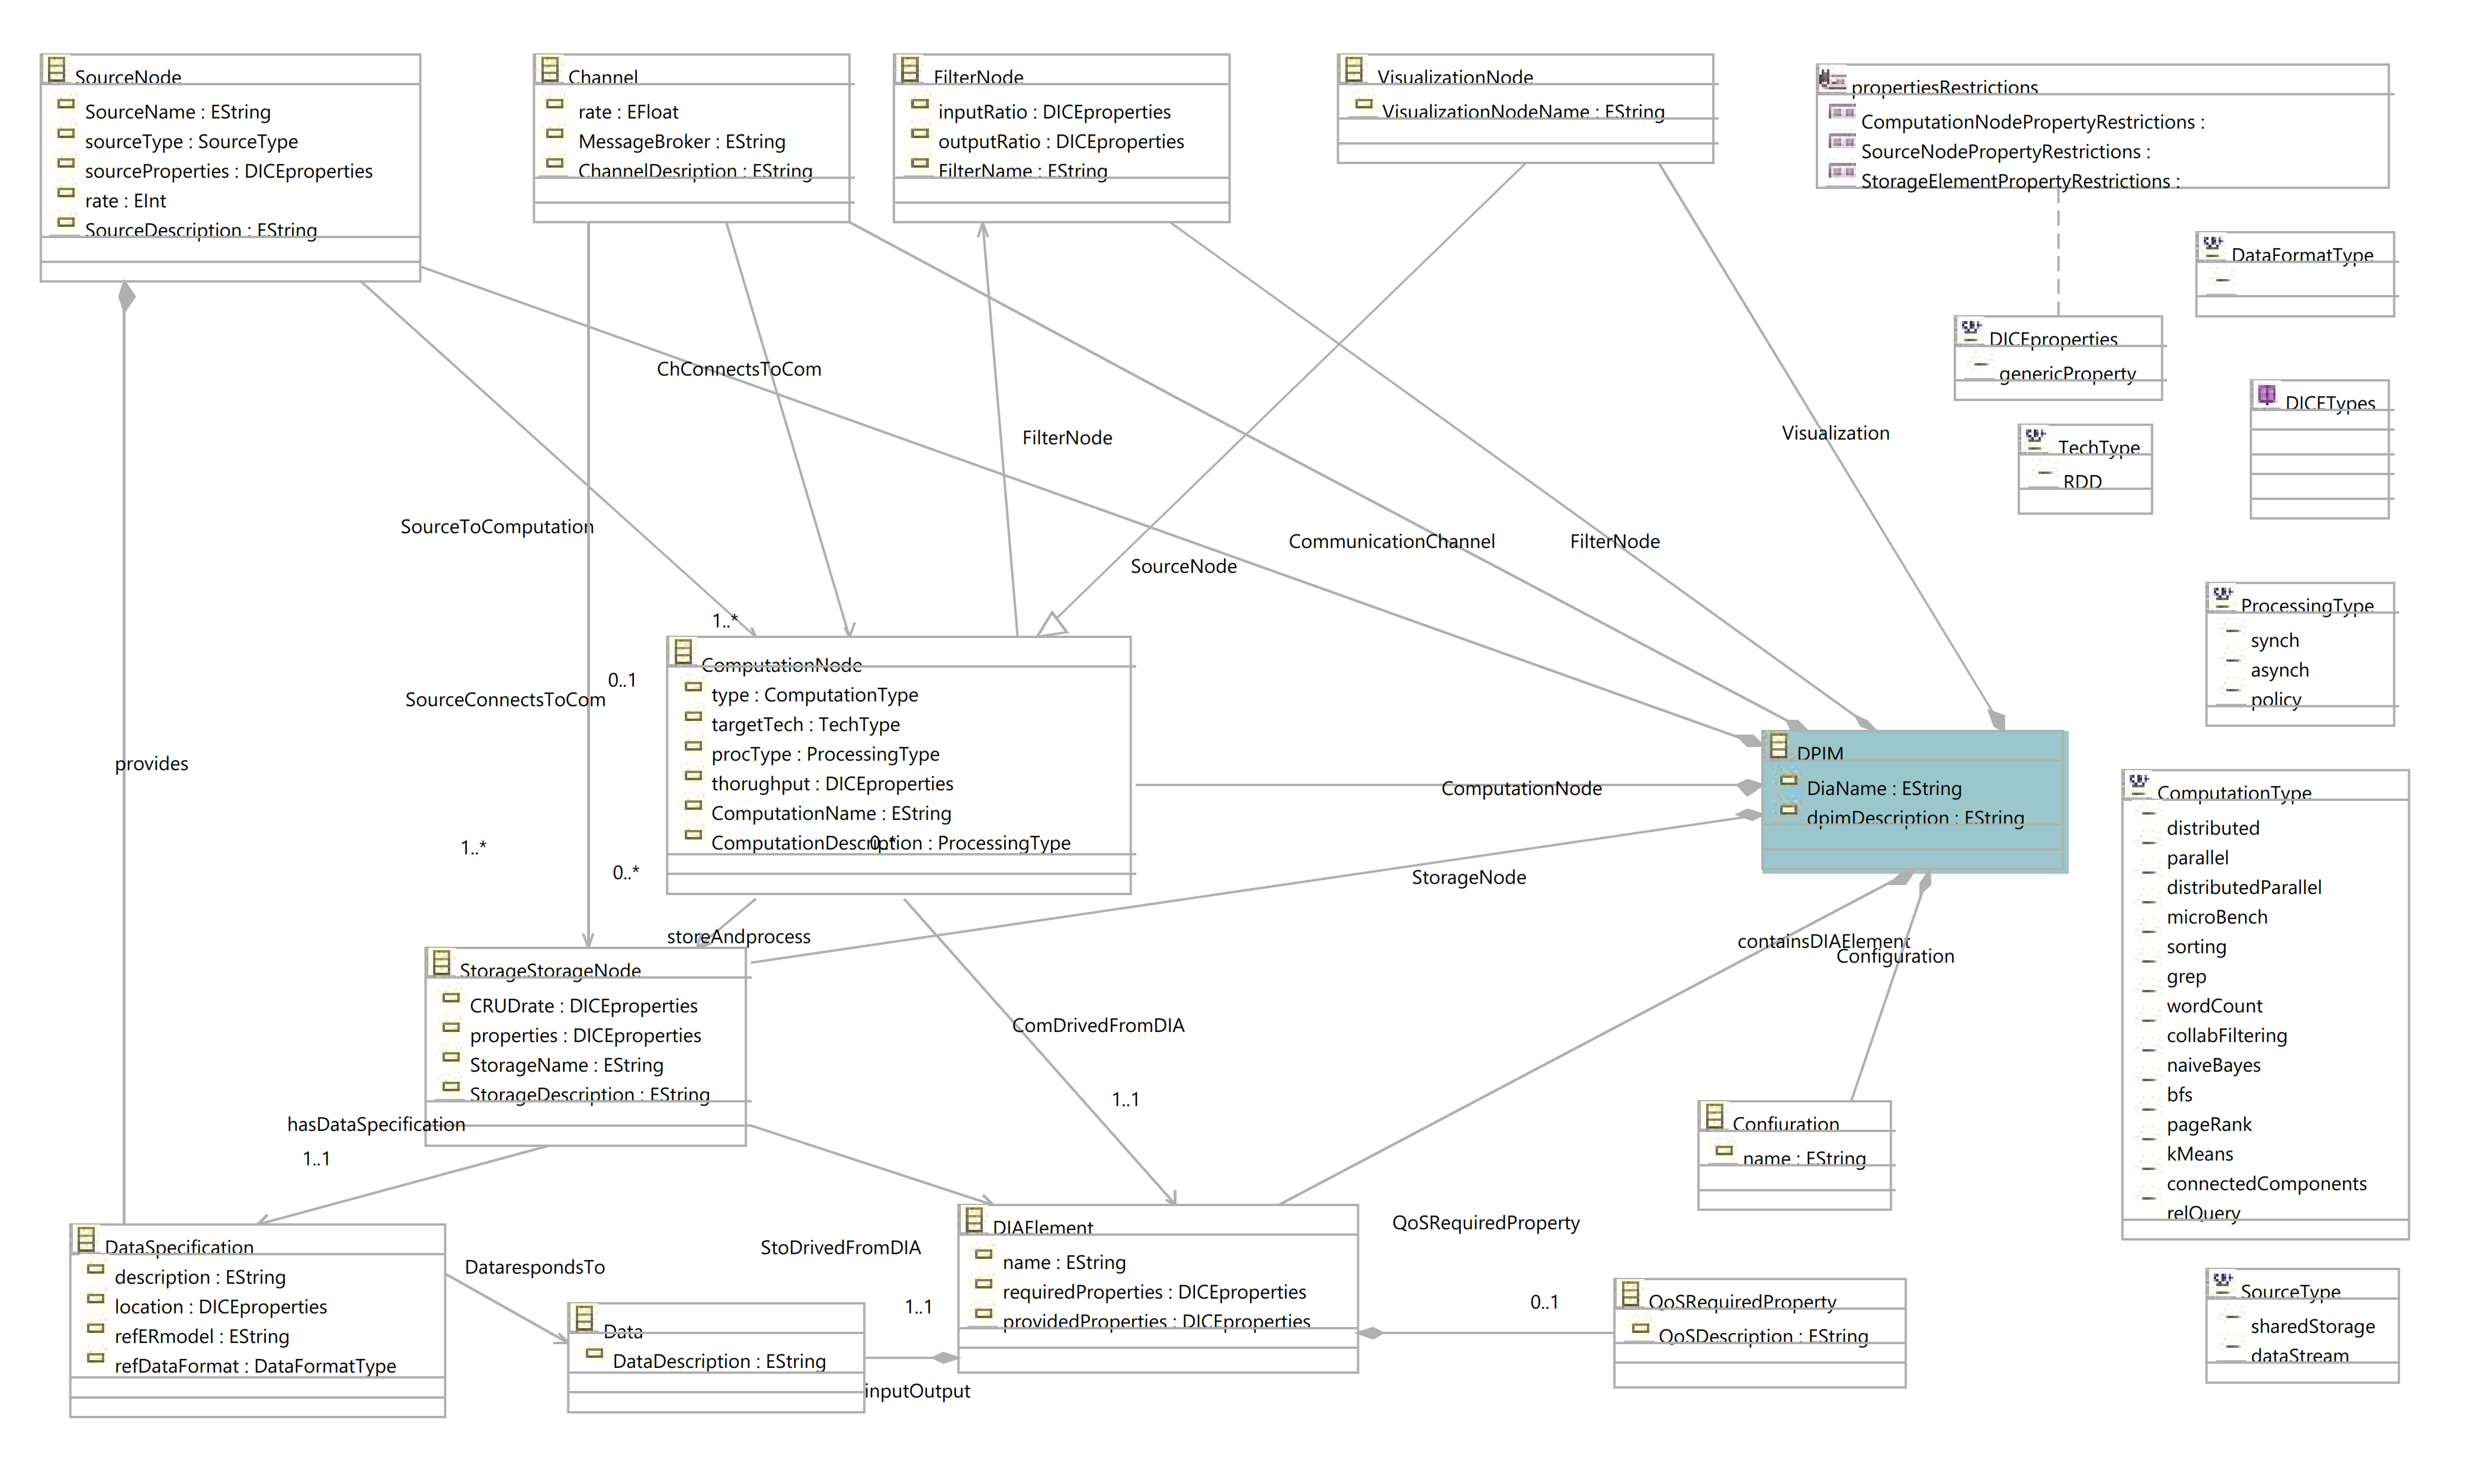
\includegraphics[width=\textwidth]{Images/11.png}
\caption{\label{fig:metamodel2}DICE DPIM metamodel in portrait form.}
\end{figure}


\subsection{Product perspective}

\subsubsection{User interfaces}

\begin{itemize}
	\item A new user should be able to make an account, without training, in less than 10 minutes
	\item The number of steps requested to user in "appointment creation" should be less than 5
	\item User should be allowed to access system functions from mobile devices such as smart-phone and tablets
	\item User should be allowed to access system functionalities from PC
	\item UI for mobile devices should adapt to different screen sizes (from 5 to 11 inch)
	\item There shouldn't be need of training for new user to learn all application functionalities offered by UI
\end{itemize}
\subsubsection{System interfaces}

System have to communicate with external services, from public transportation means to map services. In order to guarantee future support to new services, also outside Milan area, it ought to be useful a modular, flexible but also extendible approach on the building of external interface. In the following part of the paragraph it will be shown a list of logic operation that should be accomplished by external services APIs in order to be interfaced and employed by the system.

\begin{itemize}
	\item Train services and trams
	\subitem Looking for station list
	\subsubitem System request: station list
	\subsubitem Service response: list of station with locations
	
	\subitem Looking for train/tram
	\subsubitem System request: departure and arrival stations, departure time
	\subsubitem list of possible rides, cost of travel, times of leaving and arrival (at least 1 list's element)
	
	\item Taxi
	\subitem Looking for taxi
	\subsubitem System request: departure position and time
	\subsubitem Service response: disponibility and (hourly or journey cost)
	
	\item Bike sharing
	\subitem Looking for service parking spot
	\subsubitem System request: spaces
	\subsubitem Service response: list of spaces with available bicycles
	\subitem Looking for fees
	\subsubitem System request: fees
	\subsubitem Service response: hourly fee
	
	\item Map services
	\subitem System should be able to retrieve the nearest address given GPS coordinates and vice-versa by these services.
	\subitem Map services should be able to generate a route between two given address on system request.
	\subitem System should be allowed to download a portion of map.
	
	\item Weather forecast service
	\subitem Request forecast
	\subsubitem System request: forecast for a specific location and time
	\subsubitem Service response: weather conditions and temperature for requested locality and time
	
	
\end{itemize}

\subsubsection{Software interfaces}

In order to ship a complete functional software, at least for the city of Milan, a list of required supported external APIs is provided in this paragraph.

\begin{itemize}
	\item Trenitalia
	\subitem Name: “Informazioni-Treni-Italiani”
	\subitem Description: unofficial API for Trenitalia, further details on source
	\subitem Version: testing
	\subitem Source: \url{https://github.com/Razorphyn/Informazioni-Treni-Italiani}
	
	\item ATM
	\subitem Name: “localizzazione delle fermate delle linee urbane di superficie”
	\subitem Description: list of metro stops and hours in data-sheet version, regularly updated
	\subitem Version: 29/12/2015
	\subitem Source: \url{http://dati.comune.milano.it/}
	
	\item Bike Sharing
	\subitem Name: “Mobilità: localizzazione delle rastrelliere per il bike sharing”
	\subitem Description: list of bikesharing areas in datasheet version, regularly updated
	\subitem Version: 05/12/2016
	\subitem Source: \url{http://dati.comune.milano.it/}
	
	\item Taxi
	\subitem Name: “appTaxi | Developers”
	\subitem Description: restricted API to book or calculate prices for a ride
	\subitem Version: rolling
	\subitem Source: \url{www.apptaxi.it/developers/}
	
	\item Weather
	\subitem Name: “Open Weather Map API”
	\subitem Description: open API to get weather conditions for a location
	\subitem Version: rolling
	\subitem Source: \url{https://openweathermap.org/api}
	
\end{itemize}
\subsection{Product functions}

It has been selected a set of functionalities, on one hand in order to provide to user a service that focus on easy of use, automation and simplification of user processes and interactions with the system, on the other hand allowing him to freely compose complex schemes of constraints in the choice of travel routes.

\subsubsection{Preference profile creation}
A logged user should be able to create some types of constraints (flexible launch, disabilitation of transport means, set pauses from transport and maximum travelling distance by types of transport mean). He should also be allowed to create many different preferences profiles, that are logical containers for sets of user preferences. These profiles can be applied to single appointments personalizing the research of a routes. Preferences with unspecified profiles belongs to “default” profile and they will ever be considered as constraint for route generation.

\subsubsection{Appointment insertion}

A user can register an appointment providing a description, a date, a time of begin and end. Beside, a registered user can optionally add a list of preferences profiles. The appointment shouldn’t conflict with others of the same user, so if it happens, it will be rejected. Accepted appointment have to be processed, and route options prompted to user.

\subsubsection{Appointment modification}

A user can modify any detail of a previous inserted appointment. If the user is logged into the system, all modifications have to be synchronized with user account.
Finally, system should provides new routes for reaching the modified appointment, deleting previous saved routed linked with the old one.

\subsubsection{Change travel route}

A user can choose to change a saved route. In this case, system will delete user current selected saved route and it will provides new routes to user.

\subsubsection{Route choice}

When requested, the system have to generate routes to reach appointment according to registered user preferences profiles and the previous appointment. System will provide a route that will minimize distance, another one minimizing duration and others minimizing carbon footprint or number of changes.

\subsubsection{User Registration}

User can choose to register an account into the system through MA indicating a valid email address, a secure password, name, surname and fiscal code. 

\subsubsection{User login}

A registered user can log in using phone number and sms verification process or by email and password.



\subsection{User characteristics}

It’s possible to divide application users into two groups:

\begin{itemize}
	\item Unregistered
	\subitem He can access some app features, including appointment registration and route choices
	\item Registered
	\subitem He can access all the feature set that system can provide, so all the functionality provided to unregistered user, plus the possibility to set profiles of preferences, synchronization and backup of user data and preferences. This user can also receive weather forecast update.
\end{itemize}

The user of this system is not required to have IT skills.

\subsection{Assumptions}

{GET FROM EXTERNAL DOC}


%------------------------------------------------------------------------------------------------------------------------------------------------
\clearpage
{\color{Blue}{\section{Specific Requirements}}}
\label{sect:requirements}
Organize this section according to the rules defined in the project description. 


%------------------------------------------------------------------------------------------------------------------------------------------------
\clearpage
{\color{Blue}{\section{Formal Analysis Using Alloy}}}
\label{sect:alloy}
Organize this section according to the rules defined in the project description. 


%------------------------------------------------------------------------------------------------------------------------------------------------
\clearpage
{\color{Blue}{\section{Effort Spent}}}
\label{sect:effort}

\subsection{Fiorillo}

\begin{tabular}{|c|c|}
	\hline
8/10/2017	& 45m \\ 
	\hline 
11/10/2017	& 45m \\ 
	\hline 
12/10/2017	& 1h20m \\ 
	\hline 
13/10/2017	& 1h \\ 
	\hline 
15/10/2017	& 2h \\ 
	\hline 
23/10/2017	& 1h15m \\ 
	\hline 
24/10/2017	& 30m \\ 
	\hline 
26/10/2017	& 2h15m \\ 
	\hline 
28/10/2017	& 30m \\ 
	\hline
29/10/2017	& 3h \\ 
	\hline
TOT			& 13h20m \\

\end{tabular} 

\subsection{Daverio}

\begin{tabular}{|c|c|}
	\hline
	2/10/2017	& 30m \\ 
	\hline 
	4/10/2017	& 40m \\ 
	\hline 
	7/10/2017	& 30m \\ 
	\hline 
	10/10/2017	& 2h20m \\ 
	\hline 
	14/10/2017	& 1h40m \\ 
	\hline 
	18/10/2017	& 3h \\ 
	\hline 
	20/10/2017	& 45m \\ 
	\hline 
	21/10/2017	& 1h20m \\ 
	\hline 
	25/10/2017	& 1h45m \\ 
	\hline 
	27/10/2017	& 7h45m \\ 
	\hline 
	28/10/2017	& 9h30m \\ 
	\hline
	29/10/2017	& 16h45m \\ 
	\hline
	TOT			& 47h30m \\

\end{tabular}


%------------------------------------------------------------------------------------------------------------------------------------------------
\clearpage
\addcontentsline{toc}{section}{References}
\bibliographystyle{plain}
\bibliography{main}
%------------------------------------------------------------------------------------------------------------------------------------------------




\end{document}
